%parallelogram with base and height marked

\documentclass[tikz,border=10pt]{standalone}
\usepackage{tikz}
\usetikzlibrary{arrows.meta}

\begin{document}
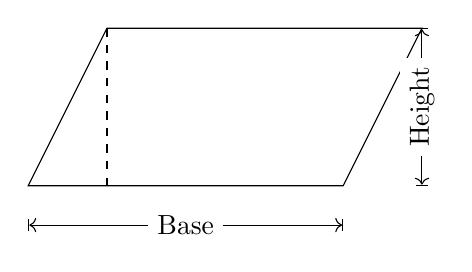
\begin{tikzpicture}

% Draw parallelogram
\draw (0,0) -- (4,0) -- (5,2) -- (1,2) -- cycle;

% Draw base dimension
\draw[|<->|] (0,-0.5) -- (4,-0.5) node[midway,fill=white] {Base};

% Draw height dimension
\draw[|<->|] (5,2) -- (5,0) node[midway,fill=white,rotate=90] {Height};

% Draw dashed height line
\draw[dashed] (1,2) -- (1,0);

\end{tikzpicture}
\end{document}